
Naturally, we would like to reduce the number of distance queries while maintaining the same distortion. However, the matching-based approach requires first obtaining a sufficiently good solution to the $k$-center problem and then mapping it to a feasible solution of the fair $k$-center problem. If we stick to this approach, we need to reduce the number of queries required to find a $2$-approximate solution for $k$-center, improving upon the results of~\citet{burkhardt2024low}; which, to our best knowledge, is still an open problem.

This motivates the following \emph{less ambitious}, yet still meaningful, question: \emph{Can we design a deterministic constant distortion algorithm for the ordinal fair $k$-center problem that uses $o(k^2)$ distance queries?}
In this section, we design such an algorithm, answering it in the affirmation. The algorithm we design starts from Burkhardt et al.'s $4$-distortion $k$-center algorithm~\cite{burkhardt2024low}, which uses only $2k$ distance queries. For completeness, we restate the result in Theorem~\ref{theorem:ordinal-k-center-algorithm-smaller-queries}.

\begin{theorem}[Theorem 3.3~\cite{burkhardt2024low}]
    \label{theorem:ordinal-k-center-algorithm-smaller-queries}
    There exists a deterministic $4$-distortion algorithm for $k$-center that makes $2k$ distance queries. 
\end{theorem}

Succinctly, we denote by \bcfrss the algorithm of \citet{burkhardt2024low} corresponding to~\Cref{theorem:ordinal-k-center-algorithm-smaller-queries}.
The main challenge consists of two parts: (i) finding a $\hat{\ell}$ such that mapping the solution $T_{\hat{\ell}}$ to the conventional $k$-center without the fairness constraints to the feasible solution $S$ according to bipartite matching obtains a $5$-approximation result; (ii) regarding the bipartite matching part, we need to adapt their algorithm to the ordinal model that can efficiently construct the bipartite graph $H^{\hat{\ell}}_{\lambda}$ with the smallest possible $\lambda$ that admits a left-perfect matching, given only access to ordinal information and a limited number of distance queries.
We will show that both parts can be achieved with significantly fewer queries than the naive $\bigO(k^2)$ bound.

The pseudocode of our main algorithm is presented in~\Cref{alg:ordinal-fair-k-center-quality-ell}. 
We structure our analysis in two parts. 
In the first part (Section~\ref{sec:4-approximate-k-center-algorithm}--\ref{sec:finalphase}), we present our algorithm, which proceeds in three phases. 
For each phase, we analyze the number of calls to costly subroutines (measured in terms of distance queries) needed and establish the distortion guarantee of the algorithm.
In the second part (Section~\ref{sec:evaluating-the-predicate}--\ref{section:finding-minimum-lambda}), we derive precise bounds on the query complexity of these subroutines, and put everything together to obtain the query complexity of the whole algorithm.
Next, we start with a high-level summary of the analysis.
\subsection{Overview}
\sbpara{\large Part $1$: The algorithm}

\sbpara{Initial phase: } In line~\ref{algo:init}, we compute a set $\InitSolSet$ of $k$ centers using \citet{burkhardt2024low}'s $4$-distortion algorithm (\Cref{theorem:ordinal-k-center-algorithm-smaller-queries}) that takes $2k$ distance queries.

\sbpara{Main Phase: } (lines~\ref{algo:pred}-\ref{algo:mainend})
This is the crucial phase of our algorithm and it starts by defining the predicate $\mathsf{P}(\ell) ~\equiv~ \bigl( 4\,\lambda_{\ell} \leq \cost(\InitSolSet_{\ell}) \bigr)$. 
This phase relies on the fact that, with respect to $\ell$, $\lambda_{\ell}$ is non-decreasing and $\cost(\InitSolSet_{\ell})$ is non-increasing (\Cref{lemma:monotonicity-properties-of-lambda-ell}). 
    Based on the monotonicity properties, we note that the predicate $\mathsf{P}(\ell)$ is monotone in $\ell$, it is initially true and becomes false after some $L$.
    The goal of the algorithm is to output $\hat{\ell}$ such that $\lambda_{\hat{\ell}} \leq \cost(\OptSolSet)$ and $\cost(\InitSolSet_{\hat{\ell}}) \leq 4\, \cost(\OptSolSet)$.
    Considering the corner cases, the mainphase itself is divided into two parts.

\noindent (i) \textit{Corner-cases} part (lines~\ref{algo:base1}-\ref{algo:basek}):
This part corresponds to the corner cases of the predicate  $\mathsf{P}(\ell) ~\equiv~ \bigl( 4\,\lambda_{\ell} \leq \cost(\InitSolSet_{\ell}) \bigr)$ defined in~\cref{algo:pred}. 
If $P(1)$ is false then it implies case (a) of~\Cref{lemma:monotonicity-of-lambda-and-cost-init-sol-set} holds, and hence, $\cost(\InitSolSet_{1}) \leq 4\,\lambda_{1} \leq 4\,\cost(\OptSolSet)$. 
On the other hand, if $P(k)$ is true then it implies case (b) of~\Cref{lemma:monotonicity-of-lambda-and-cost-init-sol-set} holds, and hence $4\,\lambda_{k} \leq \cost(\InitSolSet_{k}) \leq 4\,\cost(\OptSolSet)$.  

\noindent(ii) \textit{Binarysearch part} (lines~\ref{algo:binstart}-\ref{algo:binend}): In this part, the algorithm performs a binary search on $\{2,\dots, k-1\}$ to find the largest $L$ such that $\mathsf{P}({L})$ is true, but $\mathsf{P}({L}+1)$ is false. 
Furthermore, according to (c) of \Cref{lemma:monotonicity-of-lambda-and-cost-init-sol-set}, $L$ satisfies $\min \{\cost(\InitSolSet_{L}), 4 \lambda_{L+1}\} \leq 4\,\cost(\OptSolSet)$. 
Thus by setting $\hat{\ell} = L$ or $\hat{\ell} = L+1$, we have $\lambda_{\hat{\ell}} \leq \cost(\OptSolSet)$ and $\cost(\InitSolSet_{\hat{\ell}}) \leq 4\, \cost(\OptSolSet)$. 
This requires $O(\log k)$ many evaluations of the predicate $\mathsf{P}$, by binary search on $\ell$. 
To compare $\lambda_{L+1}$ and $4\,\cost(\InitSolSet_{L})$, the algorithm calls the subroutine \findlambda\ that computes $\lambda_{L+1}$ \emph{only once} as in Section~\ref{section:finding-minimum-lambda}.



\sbpara{Final Phase: } (lines~\ref{algo:finphst}-\ref{algo:finalphend}) 
In this phase, first the algorithm computes $\lambda_{\hat{\ell}}$ by calling the \findlambda\ subroutine;  the goal is to construct a $(\hat{\ell}, \lambda_{\hat{\ell}})$-projection graph $H^{\hat{\ell}}_{\lambda_{\hat{\ell}}}$ that maps the initial solution $\InitSolSet_{\hat{\ell}}$ to the feasible solution $\SolSet$.
Furthermore, we can bound $\cost(\SolSet) \leq \lambda_{\hat{\ell}} + \cost(\InitSolSet_{\hat{\ell}}) \leq 5\, \cost(\OptSolSet)$, yielding a $5$-distortion result.
We discuss the analysis in detail in in \Cref{theorem:get-feasible-solution}.


\sbpara{\large Part $2$: Query complexity}

\noindent To bound the query complexity, we need to show that given $\ell \in [k]$, how to evaluate $\mathsf{P}(\ell)$, and how to compute $\lambda_\ell$, both efficiently. 
Notice that obtaining the final solution $\SolSet$ does not induce additional queries, as the queries needed to compute $\SolSet$ have already been made when computing $\lambda_{\ell}$; i.e., when constructing the bipartite graph $H^{\ell}_{\lambda_{\ell}}$ and finding the left-perfect matching, the finial solution $\SolSet$ is implicitly obtained from $\InitSolSet_{\ell}$ through the matching.  
First, we show an efficient subroutine to evaluate $\mathsf{P}(\ell)$ for a given $\ell$ with only $\bigO(\ell \log \ell)$ queries.
For computing $\lambda_\ell$, we design a subroutine \findlambda, that uses a \mom\ subroutine, which is based on a binary search approach of finding a \emph{weighted} median of medians.
Note that there are $\ell k$ many values possible for $\lambda_\ell$, corresponding to $\ell$ elements of $\InitSolSet_\ell$, which is expensive to query. However, since we know the linear orderings of of $d(\SolMem, \Group)$ for any fix $\SolMem \in \InitSolSet_\ell$ and all $\Group \in \MultiGroupSet$ in advance, the subroutine can compute the weighted median of the medians of these orderings using only $\ell$ queries; in addition, it takes another $\ell \log k$ queries to reduce the search space. Furthermore, after each such computation, the subroutine reduces the search space by a quarter, resulting in $\bigO(k \log ^2 k)$ queries to find $\lambda_\ell$.
Therefore, the query complexity of~\Cref{alg:finding-lambda-ell} is $\bigO(k\log ^2 k)$, since the \textbf{while} loop of the main phase runs $\bigO(\log k)$ times, and each time it evaluates $\mathsf{P}$ and performs other operations, which require overall $\bigO(k\log^2 k)$ queries.



\subsection{Initial Phase}\label{sec:4-approximate-k-center-algorithm}
The first step of the algorithm is to obtain a set $\InitSolSet$ using~\citet{burkhardt2024low} algorithm, \bcfrss, from~\Cref{theorem:ordinal-k-center-algorithm-smaller-queries}, ignoring the group fairness constraints of $\Ical$.
We start our analysis by introducing the following lemma that captures the properties of $\InitSolSet$. 
For $\ell\in [k]$ and $\lambda \in \mathbb{R}_+$, recall that $H^{\ell}_{\lambda}$ is the $(\ell,\lambda)$-projection graph. Also, when $\ell \in [k]$ is fixed, $\lambda_{\ell}$ is the minimum value for which there exists a {left-perfect matching} on $H^{\ell}_{\lambda}$. 

\begin{restatable}{lemma}{lambdaellstarlowerboundsmallerqueries}
    \label{lemma:lambda-ell-star-lower-bound-smaller-queries}
    The set $\InitSolSet$ returned by \bcfrss on instance $\Ical=\ordfairkcenins$ of \ordfairkcen is
    a progressive $4$-cover for $\Ical$.
    Furthermore, for the critical index $\ell^* \in [k]$ of \OptSolSet, it holds that
    $\lambda_{\ell^*} \leq \cost(\OptSolSet)$, and $\cost(\InitSolSet_{\ell^*}) \leq 4\, \cost(\OptSolSet)$, and hence $\cost(\InitSolSet_{\ell^*}) \leq 4\lambda_{\ell^*} + \cost(\InitSolSet_{\ell^*}) \leq 5\, \cost(\OptSolSet)$.
\end{restatable}



\begin{algorithm}[]
\SetAlgoNoEnd
    \caption{$5$-Distortion Algorithm}
    \label{alg:ordinal-fair-k-center-quality-ell}
    \SetAlgoLined
    \KwIn{An instance of \ordfairkcen $\Ical=\ordfairkcenins$ }
    \KwOut{Solution $\SolSet$ to $\Ical$}

   Compute $k$ centers, \InitSolSet through Burkhardt et al.~\cite{burkhardt2024low}'s $5$-distortion algorithm (\Cref{theorem:ordinal-k-center-algorithm-smaller-queries})\label{algo:init}

   Define predicate 
    $\mathsf{P}(\ell) ~\equiv~ \bigl( 4\,\lambda_{\ell} \leq \cost(\InitSolSet_{\ell}) \bigr)$,
     for $\ell\in[k]$.\label{algo:pred}

    \tcp{Recall that $\lambda_{\ell}$ denotes the minimum $\lambda$ such that there exists a left-perfect matching on $H^{\ell}_{\lambda}$ and $\cost(\InitSolSet_{\ell})=\max_{u\in U} d(u,\InitSolSet_{\ell})$, the predicate checks whether $4\,\lambda_{\ell} \leq \cost(\InitSolSet_{\ell})$.}

    \tcp{Binary search on $\ell$ to find the largest $\ell$ such that $\mathsf{P}(\ell)$ holds.}


    \lIf{$\mathsf{P}(1)$ is false}{$\hat{\ell} \leftarrow 1$}\label{algo:base1}

    
    \lIf{$\mathsf{P}(k)$ is true}{$\hat{\ell} \leftarrow k$}\label{algo:basek}


    
    \Else{
        Set $L\leftarrow 1$ and $R\leftarrow k$\;\label{algo:binstart}
        
        \While{$L<R$}{
            $M \leftarrow \bigl\lfloor (L+R+1)/2 \bigr\rfloor$

            \lIf{$\mathsf{P}(M)$}{
                $L\leftarrow M$
            }\lElse{
                $R\leftarrow M-1$
            }
        }\label{algo:binend}
        $\lambda_{L+1} \gets \findlambda(\Ical, L+1, T_{L+1})$\;\label{algo:subph2st} %
        
        \lIf{$\cost(\InitSolSet_{L}) \leq 4 \lambda_{L+1}$}{
            $\hat{\ell}\leftarrow L$.
        }\lElse{
            $\hat{\ell}\leftarrow L+1$\label{algo:mainend}
        }
    }

    $\lambda_{\hat{\ell}}\gets \findlambda(\Ical, \hat{\ell}, T_{\hat{\ell}})$\;\label{algo:finphst}

    $\SolSet \gets $ solution obtained from~\Cref{theorem:get-feasible-solution}\;\label{algo:finalphend}

    Return $\SolSet$
\end{algorithm}





Slightly abusing the terminology, we say that $\lambda_\ell$ and $\cost(\InitSolSet_{\ell})$ are functions of $\ell$. The following lemma says that both $\lambda_{\ell}$ and $\cost(\InitSolSet_{\ell})$ are monoton in $\ell$, which is our key idea in designing binary search on $\ell$ by defining the predicate $\mathsf{P}(\ell) ~\equiv~ \bigl( 4\,\lambda_{\ell} \leq \cost(\InitSolSet_{\ell}) \bigr)$. 

\begin{restatable}{lemma}{monotonicitypropertiesoflambdaell}
    \label{lemma:monotonicity-properties-of-lambda-ell}
    Consider the set $\InitSolSet$ returned by \bcfrss. Then,    $\lambda_{\ell}$ is a non-decreasing function in $\ell$ and $\cost(\InitSolSet_{\ell})$ is a non-increasing function in $\ell$.
\end{restatable}

We put the proofs of \Cref{lemma:lambda-ell-star-lower-bound-smaller-queries} and \Cref{lemma:monotonicity-properties-of-lambda-ell} to the appendix. 
 

\subsection{Main Phase}\label{sec:mainphase}
In the \Cref{sec:4-approximate-k-center-algorithm}, 
as a direct implication of Lemma~\ref{lemma:lambda-ell-star-lower-bound-smaller-queries}, for $\InitSolSet$ obtained from \bcfrss on \ordfairkcen instance $\Ical$, we know that 
there exists an $\ell^*$ which holds that 
$\lambda_{\ell^*} \leq \cost(\OptSolSet)$ and $\cost(\InitSolSet_{\ell^*}) \leq 4\, \cost(\OptSolSet)$, where $S^*$ is an optimal solution for $\Ical$.
However, it is not clear how to find $\ell^*$ as the algorithm does not know the optimal partition $\Pi^*$ in advance. 
As a result, we opt to find an alternative $\hat{\ell}$ that satisfies $\lambda_{\hat{\ell}} \leq \cost(\OptSolSet)$ and $\cost(\InitSolSet_{\hat{\ell}}) \leq 4\, \cost(\OptSolSet)$ as well, this constitutes the main goal of this phase. 

Here we define a predicate $\mathsf{P}(\ell) ~\equiv~$ $( 4\,\lambda_{\ell} \leq \cost(\InitSolSet_{\ell}))$, for $\ell\in[k]$. 
The monotonicity of $\mathsf{P}(\ell)$ facilitates a binary search on $\ell$ to find such $L$ such that $\mathsf{P}(L)$ is true and $\mathsf{P}(L+1)$ is false.
Furthermore, we will show that either $L$ or $L+1$ is the desired $\hat{\ell}$. 
We present our algorithm in \Cref{alg:ordinal-fair-k-center-quality-ell}. 
Let us first present our main result of the phase, \Cref{lemma:binary-search-on-ell}, which states the correctness of the algorithm, and also serves as a framework for the analysis of the query complexity.


\begin{theorem}
    \label{lemma:binary-search-on-ell}
    In Algorithm~\ref{alg:ordinal-fair-k-center-quality-ell}, it holds that $\lambda_{\hat{\ell}} \leq \cost(\OptSolSet)$ and $\cost(\InitSolSet_{\hat{\ell}}) \leq 4\, \cost(\OptSolSet)$.
    In addition, the algorithm needs to evaluate the predicate at most $\lceil \log(k+1) \rceil +2$ times.
\end{theorem}


The monotonicity of $\mathsf{P}(\ell)$ relies on observation that $\lambda_{\ell}$ is a non-decreasing function in $\ell$ and $\cost(\InitSolSet_{\ell})$ is a non-increasing function in $\ell$, as in \Cref{lemma:monotonicity-properties-of-lambda-ell}.
The correctness of the output of the binary search on $\ell$ is established in \Cref{lemma:monotonicity-of-lambda-and-cost-init-sol-set}.
We leave the proof of \Cref{lemma:binary-search-on-ell} to the end of this section, and put the proof \Cref{lemma:monotonicity-of-lambda-and-cost-init-sol-set} in the appendix. 


\begin{restatable}{lemma}{monotonicityoflambdacost}
    \label{lemma:monotonicity-of-lambda-and-cost-init-sol-set}
    Let $\InitSolSet$ be the solution of \bcfrss on an instance $\Ical=\ordfairkcenins$ of \ordfairkcen, ignoring the group fairness constraints. Also, let $S^*$ be an optimal solution to $\Ical$. 
    Then, at least one of the three cases  holds:
\begin{itemize}
    \item[\textbf{(a)}] $\cost(\InitSolSet_{1}) \leq 4\,\lambda_{1}$. Moreover, in this case, $\lambda_{1} \leq \cost(\OptSolSet)$. 
    \item[\textbf{(b)}] $4\,\lambda_{k} \leq \cost(\InitSolSet_{k})$. Moreover, in this case, $\cost(\InitSolSet_{k}) \leq 4\,\cost(\OptSolSet)$. 
    \item[\textbf{(c)}] There exists an $2 \leq \ell' \leq k-1$ such that
    \[
        4\lambda_{\ell'} \leq \cost(\InitSolSet_{\ell'})
        \quad \text{and} \quad
        \cost(\InitSolSet_{\ell'+1}) \leq 4\, \lambda_{\ell'+1}.
    \]
    Moreover, in this case, we have
    \[
        \min \left\{ \cost(\InitSolSet_{\ell'}),~ 4\lambda_{\ell'+1} \right\} \leq 4\,\cost(\OptSolSet).
    \]
\end{itemize}
\end{restatable}

Next, we present the illustration of the binary search, which consists of the corner-case part and the binary search on $\ell$ part. 

\subsubsection{Corner-case part}\label{sec:basecase}
In this part, the algorithm checks if either $\mathsf{P}(1)$ is false or $\mathsf{P}(k)$ is true.
For the former case, we have that $\cost(\InitSolSet_{1}) < 4 \lambda_1$, which means $\cost(\InitSolSet_{1}) \leq 4\,\lambda_{1}$. Therefore,  case (a) of~\Cref{lemma:monotonicity-of-lambda-and-cost-init-sol-set}  holds,  hence $\lambda_1 \leq \cost(\OptSolSet)$.
In this case, the algorithm sets $\hat{\ell}=1$.
    When $P(k)$ is true, we have that case (b) of~\Cref{lemma:monotonicity-of-lambda-and-cost-init-sol-set} holds, hence it holds that $4\,\lambda_{k} \leq \cost(\InitSolSet_{k})$ and $\cost(\InitSolSet_{k}) \leq 4\,\cost(\OptSolSet)$.   In this case, the algorithm sets $\hat{\ell}=k$. In both cases, \Cref{lemma:binary-search-on-ell} is true.

\subsubsection{Binary search on $\ell$}
\label{sec:binary-search-on-ell}

To overcome the extended query complexity, we design a binary search approach on $\ell$. 
By the monotonicity of both $\lambda_{\ell}$ and $\cost(\InitSolSet_{\ell})$, the predicate, i.e., $P(\ell)$, is a non-increasing function in $\ell$. 
Namely, there exists such $L$ that $P(L)$ is true and $P(L+1)$ is false. 
Therefore, we can conduct a binary search on $\ell$ to find such $L$. 
Essentially, this case falls into case (c) of~\Cref{lemma:monotonicity-of-lambda-and-cost-init-sol-set}.
The algorithm outputs $\hat{\ell}$ as either $L$ or $L+1$: if $\cost(\InitSolSet_{L}) \leq \lambda_{L+1}$ it outputs $L$ and $L+1$ otherwise.

\smallskip 

Combining the \emph{corner-case part} and the \emph{binary search on $\ell$} part, we obtain a very good guarantee on the solution quality while using significantly fewer distance queries (as established in Section~\ref{sec:evaluating-the-predicate} and Section~\ref{section:finding-minimum-lambda}). 
We now formally prove \Cref{lemma:binary-search-on-ell}.




\textsc{Proof of~\Cref{lemma:binary-search-on-ell}.}
    Algorithm~\ref{alg:ordinal-fair-k-center-quality-ell} outputs $\hat{\ell}$ on three cases. 
    Case 1 that $P(1)$ is false, it implies that $\cost(\InitSolSet_{1}) < 4 \lambda_1$. 
    As a result, it holds true that $\cost(\InitSolSet_{1}) \leq 4\,\lambda_{1}$. 
    Since $\cost(\InitSolSet_{1}) \leq 4\,\lambda_{1}$ holds true, it implies that case (a) holds. 
    Case 2 that $P(k)$ is true directly implies case (b) holds $4\,\lambda_{k} \leq \cost(\InitSolSet_{k})$.  
    In Case 3, the algorithm conducts a binary search on $\ell$ and find the maximum $\ell$ (i.e. the $L$ in the algorithm) such that $P(\ell)$ holds. This implies case (c) holds $4\lambda_{\ell} \leq \cost(\InitSolSet_{\ell})$ and $\cost(\InitSolSet_{\ell + 1}) \leq 4\, \lambda_{\ell +1}$.
    In addition, the algorithm outputs $\hat{\ell}$ as either $L$ or $L+1$: if $\cost(\InitSolSet_{L}) \leq \lambda_{L+1}$ it outputs $L$ and $L+1$ otherwise.
    In all the three cases, the algorithm outputs $\hat{\ell}$ such that $\lambda_{\hat{\ell}} \leq \cost(\OptSolSet)$ and $\cost(\InitSolSet_{\hat{\ell}}) \leq 4\, \cost(\OptSolSet)$ holds.
    In addition, the algorithm needs to evaluate the predicate at most $\lceil \log(k+1) \rceil$ this is because each time in the binary search, the search space is halved.
\hfill\qed


\subsection{Final Phase}\label{sec:finalphase}
Once the algorithm computes $\hat{\ell}$ that satisfies~\Cref{alg:finding-lambda-ell}, it computes $\lambda_{\hat{\ell}}$ in~\Cref{algo:finphst}.
Next in~\Cref{algo:finalphend}, it computes a feasible solution $\SolSet_{\hat{\ell}}$ by mapping the left-perfect matching on $H^{\hat{\ell}}_{\lambda_{\hat{\ell}}}$ from $\InitSolSet_{\hat{\ell}}$ to $\MultiGroupSet$,  and obtain a $5$-approximate solution to the ordinal fair $k$-center problem.
We leave the proof to the appendix in the full version of the paper. 
 
\begin{restatable}{theorem}{getfeasiblesolution}
    \label{theorem:get-feasible-solution} 
    Given $\hat{\ell} \in [k]$ and $\lambda_{\hat{\ell}}$, we can construct the left-perfect matching on the $(\hat{\ell}, \lambda_{\hat{\ell}})$-projection graph $H^{\hat{\ell}}_{\lambda_{\hat{\ell}}}$, to obtain a feasible solution $\SolSet$ as follows:
    suppose that $s \in \InitSolSet_{\hat{\ell}}$ is matched to $\MultiGroup_i$ in the left-perfect matching, 
    add the point in $\MultiGroup_i$ that is closest to $s$ into $\SolSet$. 
    We then add one arbitrary point from the groups that are not matched from $\InitSolSet_{\hat{\ell}}$. 
    The solution $\SolSet$ is a feasible solution for the fair $k$-center problem with distortion at most $5$.
\end{restatable}






\subsection{Evaluating the predicate} \label{sec:evaluating-the-predicate}
Now, we analyze how many distance queries are needed to evaluate the predicate $\mathsf{P}(\ell) ~\equiv~$ $( 4\,\lambda_{\ell} \leq \cost(\InitSolSet_{\ell}))$ for any given $\ell \in [k]$. 
A naive way to evaluate the predicate is to compute both $\lambda_{\ell}$ and $\cost(\InitSolSet_{\ell})$, and compare the values. 
However, computing each $\lambda_{\ell}$ is costly, as we later show in \Cref{section:finding-minimum-lambda} which costs $\bigO(k \log^2 k)$ distance queries and leading to $\bigO(k^3)$ distance queries in total.
An alternative approach is to view the predicate in its equivalent formulation, i.e., $P(\ell) ~\equiv~$ $( \lambda_{\ell} \leq \frac{1}{4} \cdot \cost(\InitSolSet_{\ell}))$.
This formulation essentially checks whether there exists a left-perfect matching on the $(\ell, \frac{1}{4} \cdot \cost(\InitSolSet_{\ell}))$-projection graph $H^{\ell}_{\frac{1}{4} \cdot \cost(\InitSolSet_{\ell})}$.

With this equivalent formulation, we note that evaluating the predicate only costs the distance queries in two parts. 
The first part is to construct the $(\ell, \frac{1}{4} \cdot \cost(\InitSolSet_{\ell}))$-projection graph, which takes at most $\ell \log(k)$ distance queries, we present the result in \Cref{lemma:construct-graph-queries} with more general setting on $\lambda$.  
The second part is to compute the cost of $\InitSolSet_{\ell}$, which takes $\ell$ distance queries to compute. 
Combining the two parts, we get \Cref{lemma:evaluate-predicate-queries}.  
We leave the proof to the appendix.

\begin{restatable}{lemma}{constructgraphqueries}
    \label{lemma:construct-graph-queries}
    Constructing the $(\ell, \lambda)$-projection graph $H^{\ell}_{\lambda}$ takes at most $\ell \log(k)$ distance queries, for any arbitrary $\lambda \geq 0$ and a fixed $\ell$.
    
\end{restatable}


\begin{restatable}{lemma}{evaluatepredicatequeries}
    \label{lemma:evaluate-predicate-queries}
    Given $\ell \in [k]$, it takes at most $\ell \log(k) + \ell$ distance queries to evaluate the predicate $\mathsf{P}(\ell)$.
\end{restatable}


\subsection{Computing $\lambda_\ell$}
\label{section:finding-minimum-lambda}
\begin{figure*}[htbp]
    \centering
    \begin{tabular}{p{0.45\textwidth}p{0.45\textwidth}}
        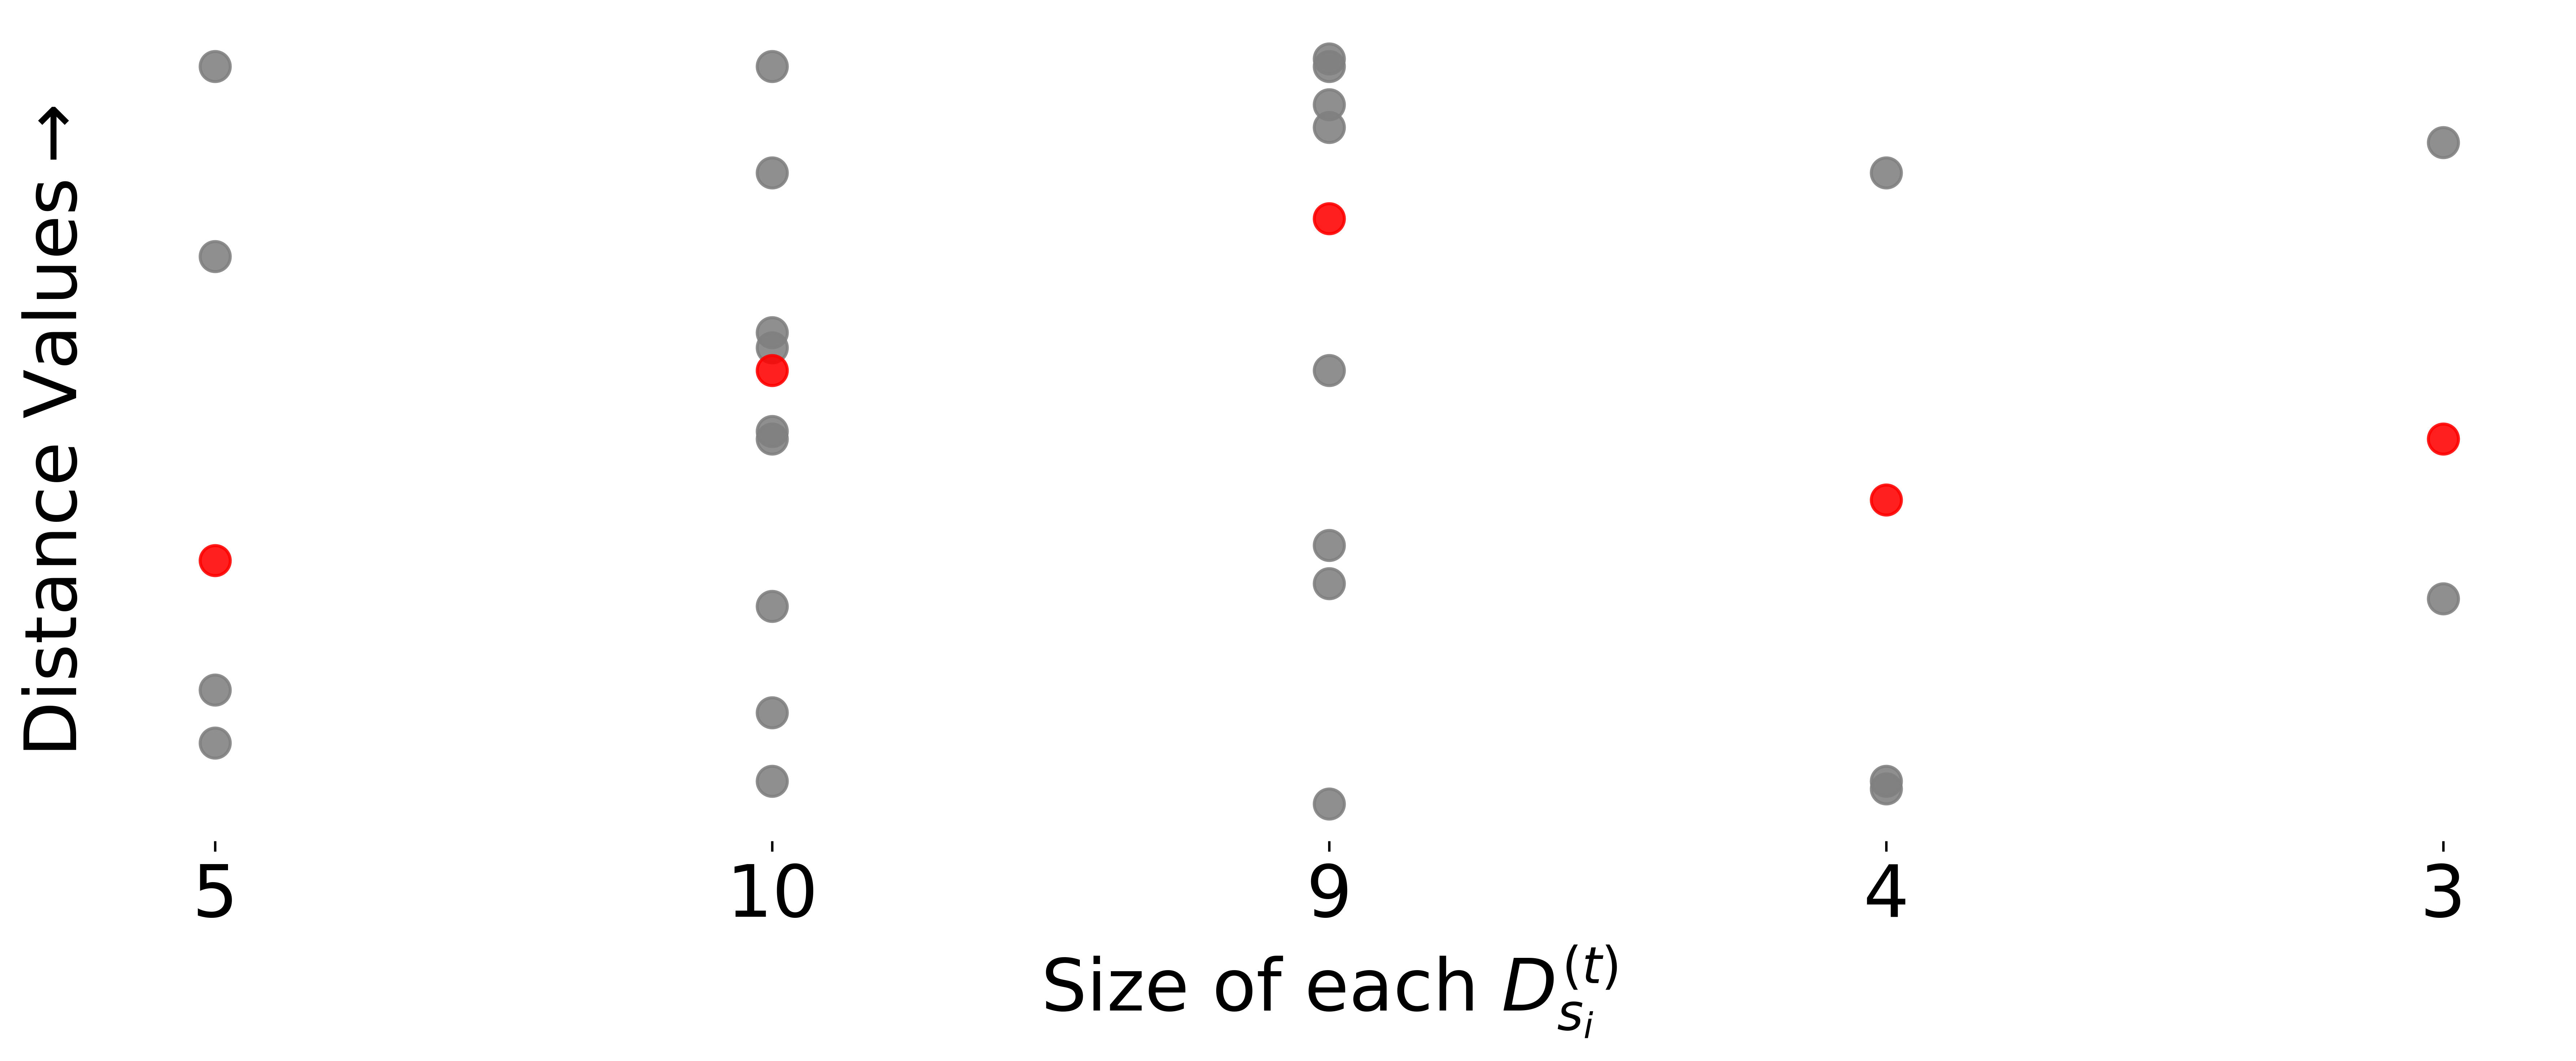
\includegraphics[width=0.45\textwidth]{sets_visualization.png} &
        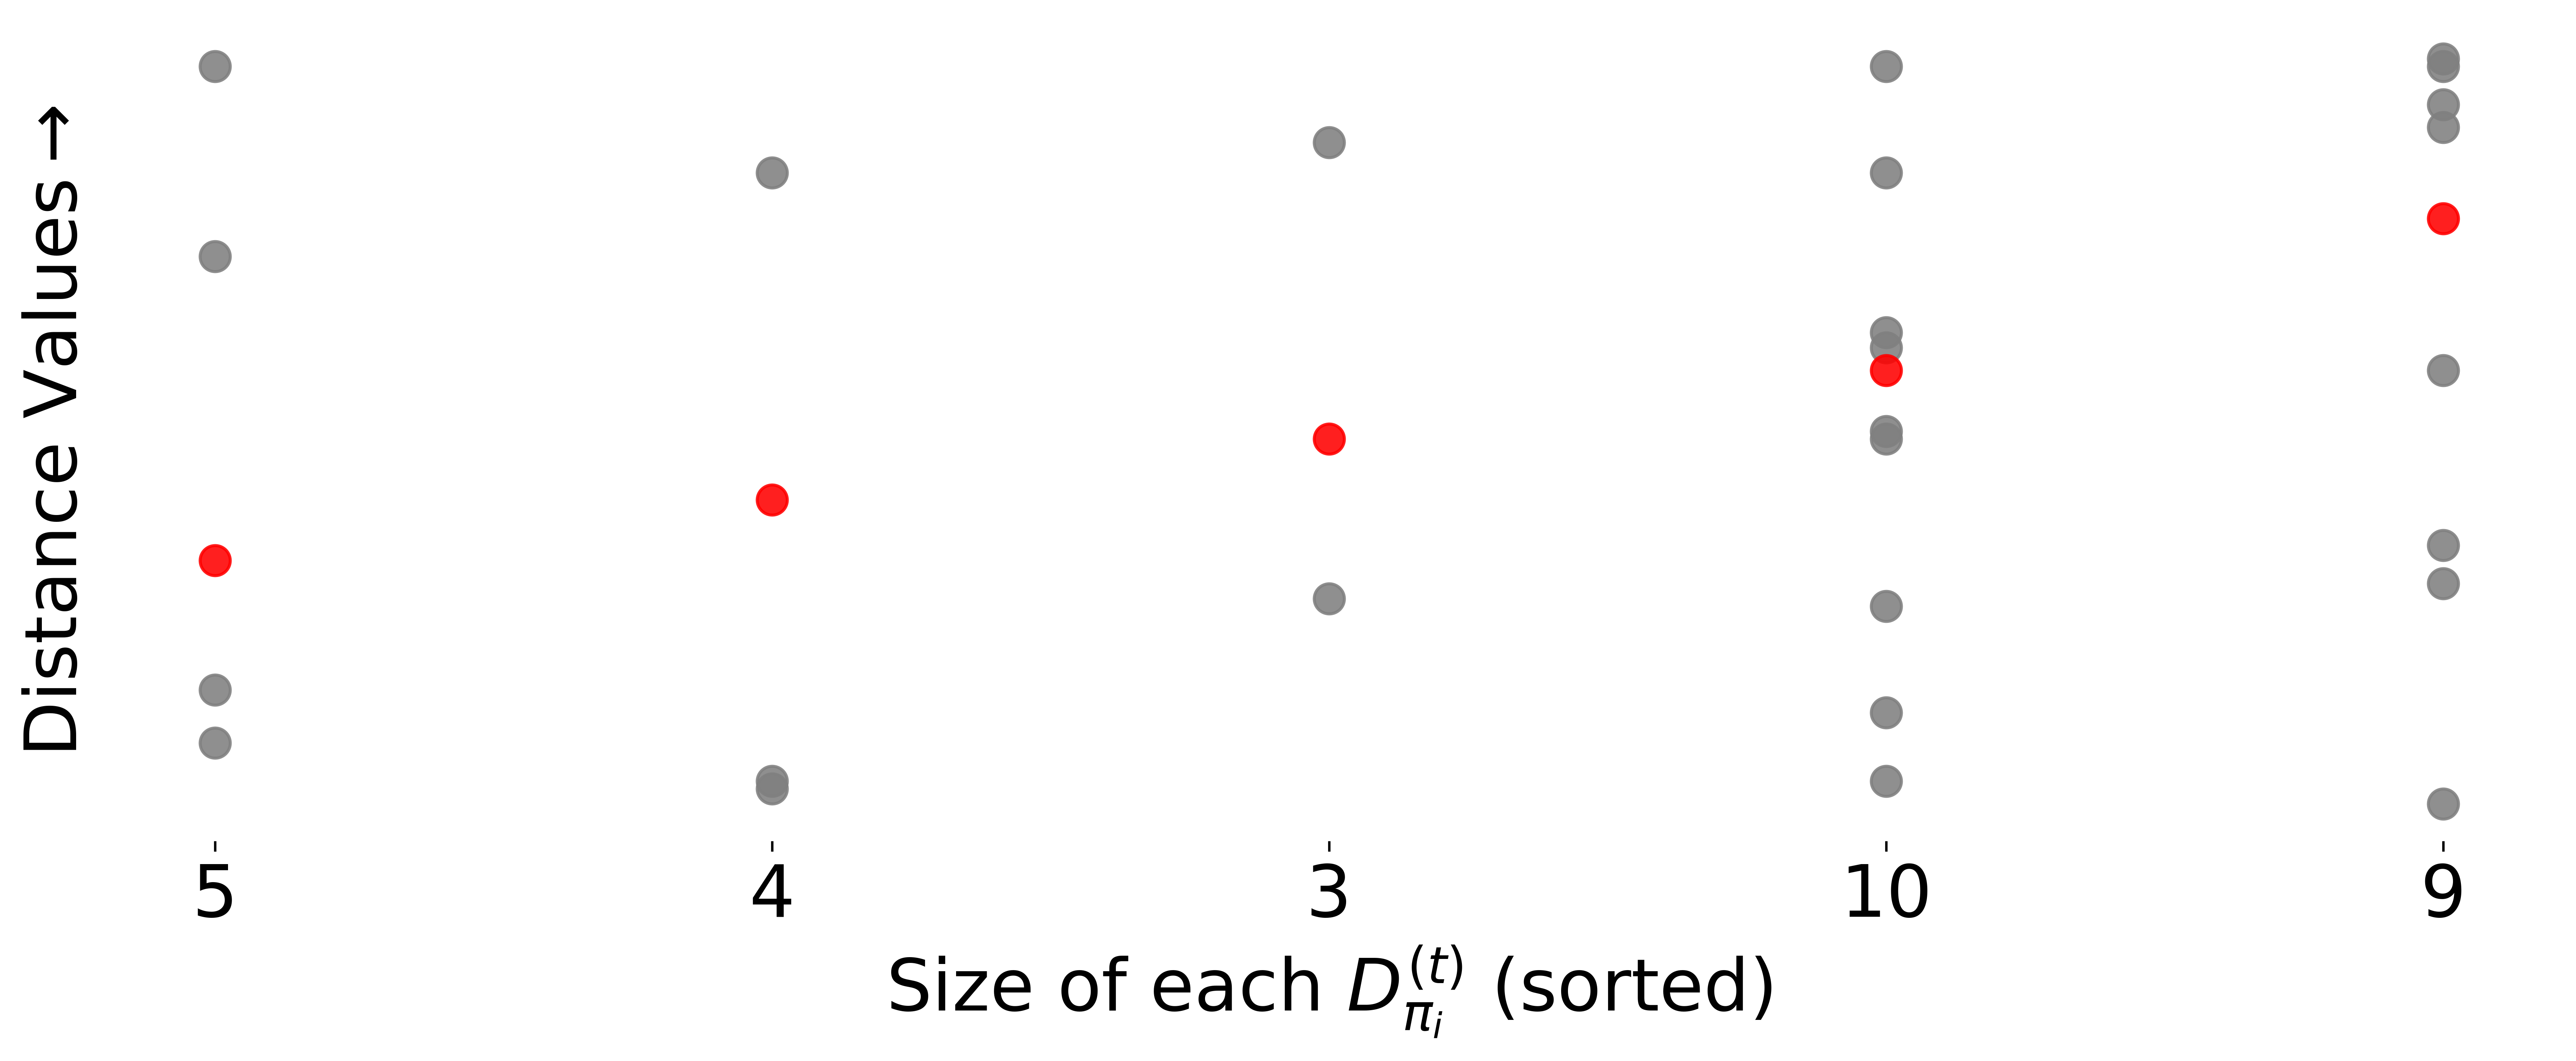
\includegraphics[width=0.45\textwidth]{sets_visualization_sorted.png} \\
        (a) Each column visualizes the distance values in $D_{s_i}^{(t)}$ for $i \in [\ell]$. The medians $\MED(D_{s_i}^{(t)})$ are marked in red. &
        (b) Sorting the $\{D_{s_i}^{(t)}\}_{i \in [\ell]}$ so that the medians $\MED(D_{s_i}^{(t)})$ are ordered increasingly from left to right. \\
        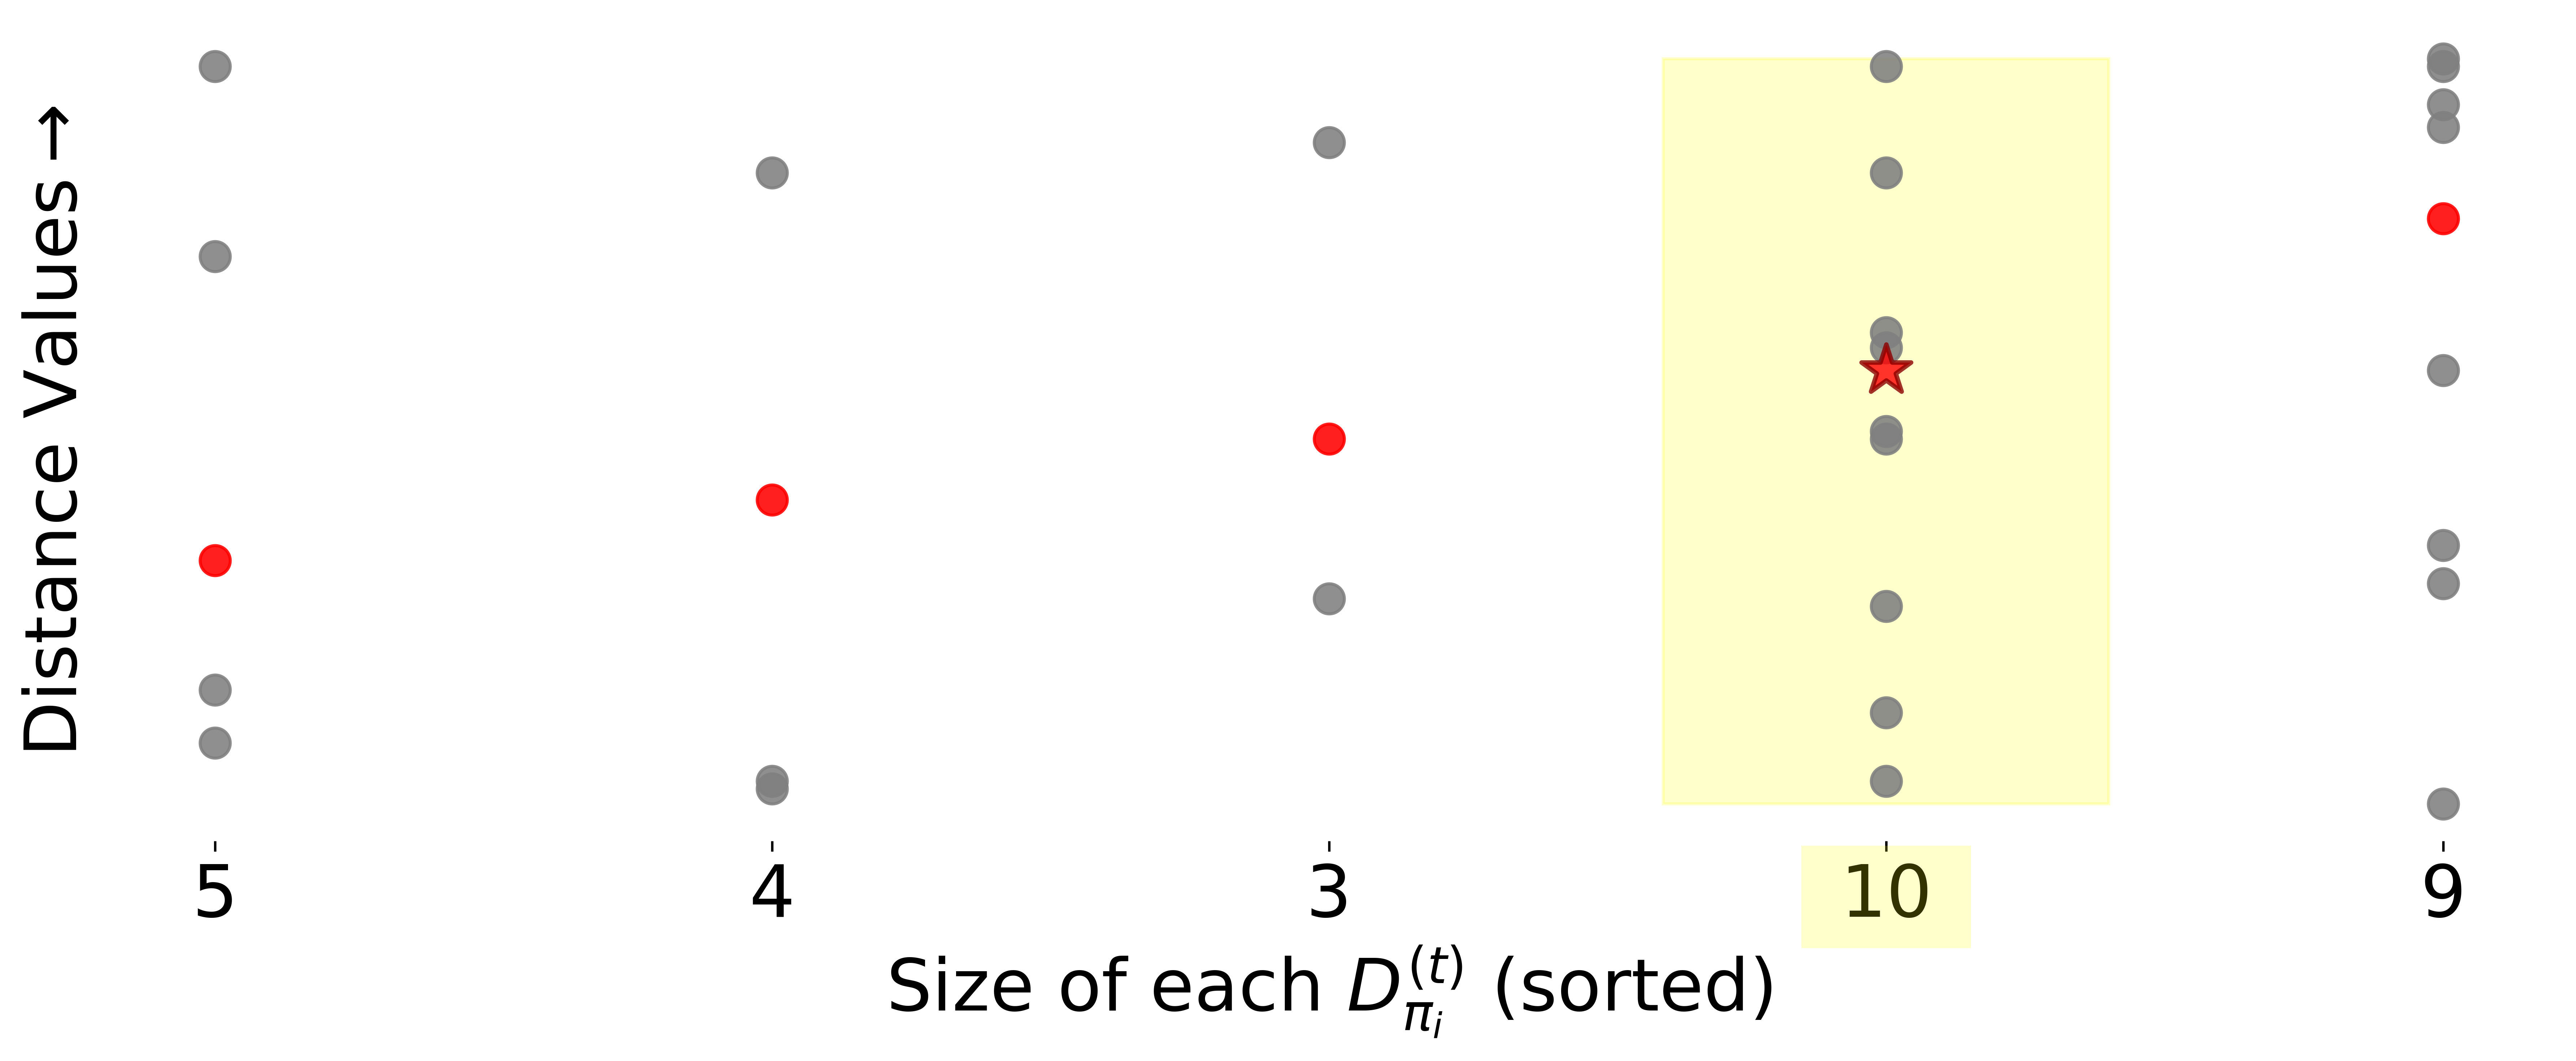
\includegraphics[width=0.45\textwidth]{sets_visualization_star.png} &
        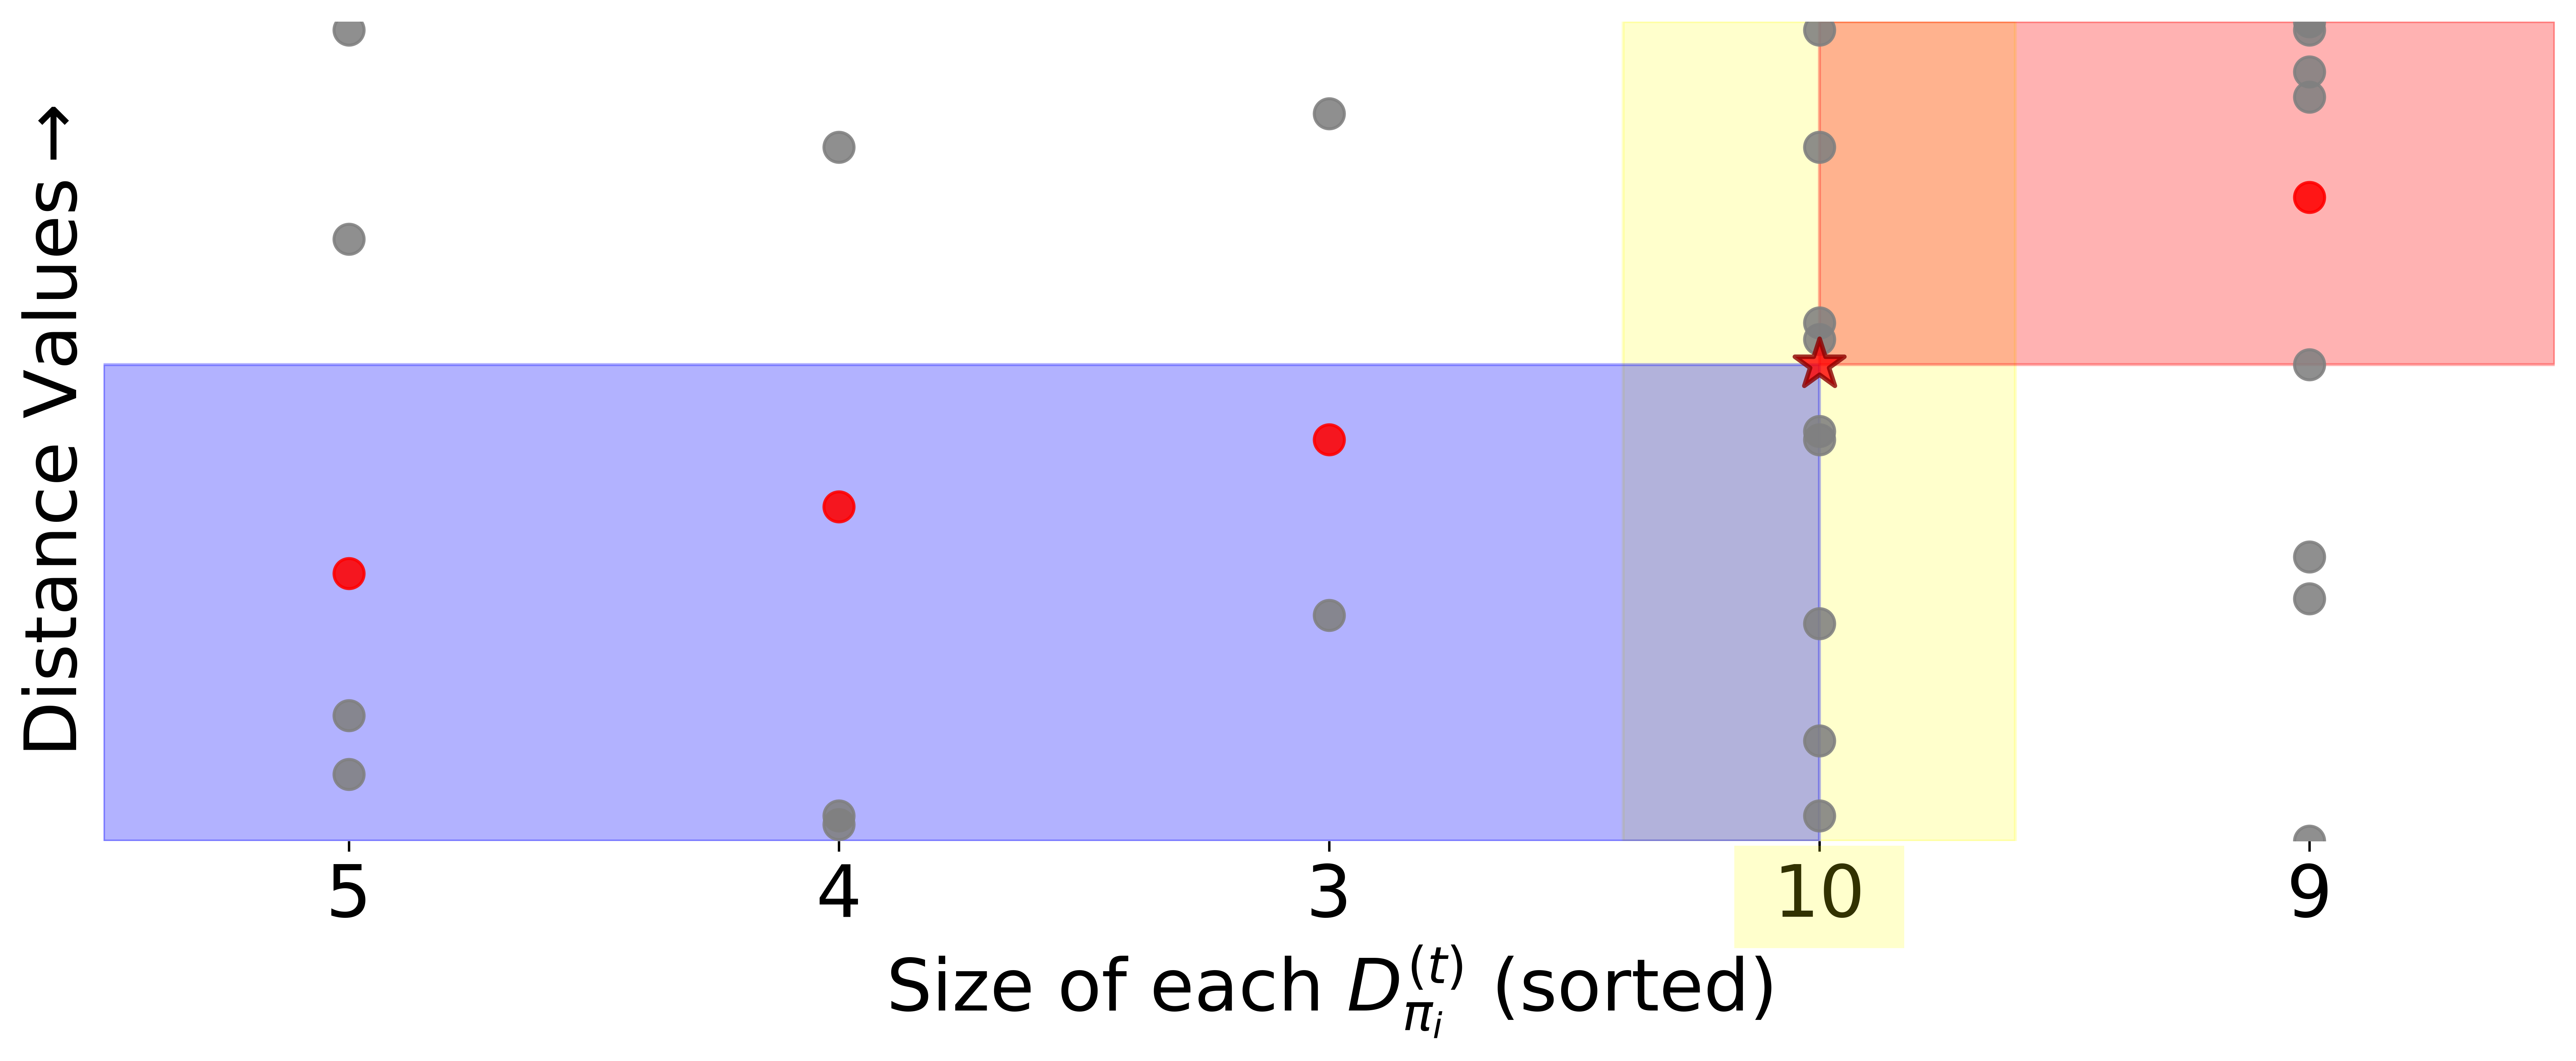
\includegraphics[width=0.45\textwidth]{sets_visualization_quadrants.png} \\
        (c) The \emph{weighted} median corresponding to the sizes of $D_{\pi_i}^{(t)}$ is selected and marked in yellow. The pivot point $\tau$ is the median of the corresponding distances. &
        (d) We observe that least $1/4$ of distance values (in red) are $\geq$ the pivot point $\tau$, and at least $1/4$ (in blue) are $\leq$ the pivot point $\tau$. \\
    \end{tabular}
    \caption{An illustration of the median-of-medians approach.} 
    \label{fig:combined_examples}
\end{figure*}

In \Cref{alg:ordinal-fair-k-center-quality-ell}, the algorithm needs to compute $\lambda_{\ell}$ twice, respectively in line~\ref{algo:subph2st} and line~\ref{algo:finphst}; we need an efficient way to compute $\lambda_{\ell}$ with as few distance queries as possible. 
Towards this, we propose~\Cref{alg:finding-lambda-ell} (\findlambda), that itself is based on \emph{median of medians} approach of~\Cref{alg:median-median} (\mom).
Our main result is that it takes at most $\bigO(k \log^2(k))$ distance queries to find $\lambda_{\ell}$, and we state this result in \Cref{theorem:min-lambda-with-perfect-matching}. 
We first give an overview of the algorithm and then present the proof in \Cref{theorem:min-lambda-with-perfect-matching} at the end of the section.

\begin{theorem}
    \label{theorem:min-lambda-with-perfect-matching}
    For any fixed $\ell$, Algorithm~\ref{alg:finding-lambda-ell} takes $\bigO(k \log^2(k))$ distance queries to find $\lambda_\ell$.
\end{theorem}

A naive approach to find $\lambda_{\ell}$ is to query all the distance values between the initial centers $\InitSolSet$ and all the other points, and conduct the standard binary search~\cite{gadekar2025fair}, which takes $nk$ distance queries.  
In our paper, we reduce the search space $D = \{d(\SolMem_i, \MultiGroup_j) \mid i \in [\ell], j \in [k]\}$, note that entries of $D$ is not known and need to be queried; and we reduce the distance queries by utilizing the structure of $D$.
We give an illustration of the algorithm in \Cref{fig:combined_examples}, and we give a detailed explanation in the following. 


\sbpara{Step (a)} 
Denote $\InitSolSet_{\ell} = \{\SolMem_1, \SolMem_2, \dots, \SolMem_{\ell}\}$. 
Let the search space of $D$ at $t$-th step be $D^{(t)}$, which is initialized as $D^{(0)} = D$.  
Denote $D_{\SolMem_i}^{(t)} = \{d(\SolMem_i, \MultiGroup_j) \in D^{(t)} \mid j \in [k]\}$ for each $i \in [\ell]$, which is the set of distance values between the center $\SolMem_i$ and the groups in $\MultiGroupSet$ that remain in the search space at the $t$-th step.
For any fixed $s_i$, the ordering of $D_{\SolMem_i}^{(t)} = \{d(\SolMem_i, \MultiGroup_j)\}_{j \in [k]}$ is known to the algorithm.
Denote the median of $D_{\SolMem_i}^{(t)}$ as $\MED(D_{\SolMem_i}^{(t)})$; we break tie arbitrarily.  
This only costs one distance query to obtain the median value. 

\sbpara{Step (b)}
The algorithm sorts $D_{\SolMem_i}^{(t)}$ according to the values of $\MED(D_{\SolMem_i}^{(t)})$ for any $i \in [\ell]$ in non-decreasing order, which does not cost additional distance queries.  
Let the sorted $\{D_{\SolMem_i}^{(t)}\}_{i \in [\ell]}$ be $\{D_{\pi_i}^{(t)}\}_{i \in [\ell]}$.

\sbpara{Step (c)}
Next, we find a \emph{weighted} median of the $\{\abs{D_{\pi_i}^{(t)}}\}_{i \in [\ell]}$ and denote its index as $\pidx$. 
Particularly, we need to find the $\pidx$ such that the following two conditions hold:
$\sum_{i=\pidx}^{k} \abs{D_{\pi_i}^{(t)}} \geq \frac{1}{2}\sum_{i=1}^k \abs{D_{\pi_i}^{{t}}} = \frac{1}{2} \abs{D^{(t)}}$ and $\sum_{i=1}^{\pidx} \abs{D_{\pi_i}^{(t)}} \geq \frac{1}{2}\sum_{i=1}^k \abs{D_{\pi_i}^{{t}}} = \frac{1}{2} \abs{D^{(t)}}$.
This $\pidx$ is picked according to \emph{line 3} of Algorithm~\ref{alg:median-median}.
We denote the pivot point (a weighted median-of-median) as $\tau = \MED(D_{\pi_{\pidx}}^{(t)})$. 

\sbpara{Step (d)}
The $\tau$ selected in Step (c) has a nice property that at least $1/4$ of the distance values are greater or equal to $\tau$, and at least $1/4$ of the distance values are smaller or equal to $\tau$. In this way, it helps us to reduce our search space by the factor at least $\frac{1}{4}$,
the concrete proof we present in \Cref{lemma:median-median}. 

\smallskip 

Concretely, we introduce the {binary search} based on \emph{median of medians} approach, which we present in Algorithm~\ref{alg:median-median}.
We denote $\mom(D^{(t)}, \tau^{(t)})$ as the \emph{median-of-median search} of the search space $D^{(t)}$ at the $t$-th iteration and $\tau^{(t)}$ as the \emph{current best feasible result}. 
Here, the \emph{median-of-median} is not the exact median; however, it is able to reduce the search space by a constant factor, which we show in step (c) and more formally in Lemma~\ref{lemma:median-median}.
The $\mom(D^{(t)}, \tau^{(t)})$ essentially does two things. First, it finds a pivot point $\tau$ as in line~\ref{algo:find-pivot}. Second, it constructs the bipartite graph $H^{\ell}_{\tau}$ and checks if it has a left-perfect matching: if yes, it means that $\lambda_{\ell} \leq \tau$, and $\tau$ is the current best feasible result; if no, it means that $\lambda_{\ell} > \tau$, and $\tau$ is not a feasible result, and the algorithm returns $\tau^{(t)}$ as the current best feasible result.

Next, the \Cref{lemma:reduce-search-space} shows the number of distance queries needed to construct the next search space $D^{(t+1)}$, respectively from line~\ref{algo:reduce-search-space-up} and line~\ref{algo:reduce-search-space-down} that correspond to $\lambda_{\ell} \leq \tau$ and $\lambda_{\ell} > \tau$.
Thus, the next search space $D^{(t+1)}$ consists of either all the distances that are \emph{strictly smaller than $\tau$} (since we already recorded $\tau$ as the current best feasible result) or all the distances that are \emph{strictly greater than $\tau$}. 
Using the same argument as \Cref{lemma:construct-graph-queries}, we can show for a fixed threshold $\tau$, it takes at most $\ell \log(k)$ distance queries to construct the next search space $D^{(t+1)}$, we state it in \Cref{lemma:reduce-search-space}. 
\begin{restatable}{lemma}{reducesearchspace}
    \label{lemma:reduce-search-space}
    For any fixed threshold $\tau$ and the current search space $D^{(t)}$, it takes at most $\ell \log(k)$ distance queries to find the distances that are strictly smaller than $\tau$ or the distances that are strictly greater than $\tau$.
\end{restatable}



\begin{algorithm}[]
    \SetAlgoNoEnd
    \caption{\findlambda}
    \label{alg:finding-lambda-ell}
    \SetAlgoLined
    \KwIn{An instance $\Ical$ of \ordfairkcen, $\ell \in [k]$, and $\InitSolSet_{\ell}$}
    \KwOut{$\lambda_{\ell}$}
    \tcp{Finding $\lambda_{\ell}$ using ordinal information}
    
    Let the search space be defined as a set of distance values of all the possible pairs between the centers in $\InitSolSet_{\ell}$ and the groups in $\MultiGroupSet$, i.e., $D^{(0)} = \{d(\SolMem_i, \MultiGroup_j) \mid i \in [\ell], j \in [k]\}$

    Let $\tau^{0} = \max D $ \tcp{Maximum distance value}

    \For{$t = 0, 1, \dots, \log_{\frac{4}{3}}(k \ell)$}{
    $D^{(t+1)}, \tau^{(t+1)} = \mom(D^{(t)}, \tau^{(t)})$

    \If{$D^{(t+1)}$ is empty}{
        Return $\tau^{(t+1)}$
    }
    }

\end{algorithm}

\begin{algorithm}[h]
\SetAlgoNoEnd
    \caption{The Median of Medians $\mom(D^{(t)})$}
    \label{alg:median-median}
    \SetAlgoLined
    \KwIn{$D^{(t)}$, $\tau^{(t)}$}
    \KwOut{$D^{(t+1)}$, $\tau^{(t+1)}$}

    Sort $\{D_{s_i}^{(t)}\}_{i \in [\ell]}$ in non-decreasing order according to the distance value of $\MED(D_{s_i}^{(t)})$ across $i \in [\ell]$. Here, $\MED(D_{s_i}^{(t)})$ is the median of $D_{s_i}^{(t)}$

    Denote the sorted $\{D_{\SolMem_i}^{(t)}\}_{i \in [\ell]}$ as $\{D_{\pi_i}^{(t)}\}_{i \in [\ell]}$.
    Let the size of $D^{(t)}$ be $L^{(t)}$


    \tcp{Start with $j=1$, and increment $j$ until the condition is met}

    Let $\pidx$ be the smallest $j$ such that $\sum_{i=1}^{j} \abs{D_{\pi_{i}}^{(t)}} \geq \frac{L^{(t)}}{2}$ 



    Let $\tau = \MED(D_{\pi_{\pidx}}^{(t)})$ and construct the bipartite graph $H^{\ell}_{\tau}$ \label{algo:find-pivot}

    \uIf{$H^{\ell}_{\tau}$ has a left-perfect matching}{
        $\tau^{(t+1)} = \tau$ \tcp{$\tau$ is current best feasible result}
        
        $D^{(t+1)} = \{d \in D^{(t)} \mid d < \tau \}$  \label{algo:reduce-search-space-up}
    }
    \Else{
        $\tau^{(t+1)} = \tau^{(t)}$ \tcp{$\tau^{(t)}$ is best feasible result from the previous step}
        $D^{(t+1)} = \{d \in D^{(t)} \mid d > \tau \}$ \label{algo:reduce-search-space-down}
    }
    Return $D^{(t+1)}$, $\tau^{(t+1)}$
\end{algorithm}


We state our observation from step (d) formally here that at each iteration, the search space is reduced by a constant factor. 

\begin{restatable}{lemma}{medianmedian}
    \label{lemma:median-median}
    Each invocation of Algorithm~\ref{alg:median-median} reduces the search space by at least $\frac{1}{4}$, namely, $\abs{D^{(t+1)}} \leq \frac{3}{4} \abs{D^{(t)}}$.
\end{restatable}



As a direct implication of Lemma~\ref{lemma:median-median}, we get,
\begin{corollary}
    It takes at most $\log_{\frac{4}{3}}(k \ell)$ iterations to find the minimum value of $\lambda_{\ell}$.
\end{corollary}

Now, we are ready to give a correctness proof for Algorithm~\ref{alg:finding-lambda-ell} that it indeed outputs $\lambda_{\ell}$, we state it in \Cref{theorem:correctness-of-finding-lambda-ell}. 
Our proof is by contradiction, and is an extension of the standard binary search proof. 

\begin{theorem}
    \label{theorem:correctness-of-finding-lambda-ell}
    Given $\ell \in [k]$, Algorithm~\ref{alg:finding-lambda-ell} outputs $\lambda_{\ell}$. 
\end{theorem}
\begin{proof}
    We prove by contradiction. 
    Let's make case distinctions. 
    Suppose the algorithm outputs $\lambda' > \lambda_{\ell}$; it indicates at one step, $\lambda_{\ell}$ is removed from the search space but $\lambda'$ is not. 
    Namely algorithm~\ref{alg:median-median} set a threshold $\tau$ such that $\tau \geq \lambda_{\ell}$, and $H^{\ell}_{\tau}$ does not have a left-perfect matching. 
    This is already a contradiction with the definition of $\lambda_{\ell}$. 

    Next, let us suppose the algorithm outputs $\lambda' < \lambda_{\ell}$, again it indicates that at some step $\lambda_{\ell}$ is removed from the search space but $\lambda'$ is not. 
    There are only two scenarios, the first is that at one step $t$, the algorithm sets $\tau = \lambda_{\ell}$ and finds the left-perfect matching. In this scenario, it holds that $\tau^{t'} = \lambda_{\ell}$ for any following step $t'$ after $t$. Contrary to that the algorithm outputs $\lambda'$. 
    The second is that the algorithm sets $\tau < \lambda_{\ell}$ and finds the left-perfect matching, which is not possible by the definition of $\lambda_{\ell}$. 

    Thus we conclude Algorithm~\ref{alg:finding-lambda-ell} outputs $\lambda_{\ell}$. 
\end{proof}


We are now ready to prove Theorem~\ref{theorem:min-lambda-with-perfect-matching}.

\begin{proof}[Proof of Theorem~\ref{theorem:min-lambda-with-perfect-matching}]
    The correctness of the algorithm is proved by Theorem~\ref{theorem:correctness-of-finding-lambda-ell}.
    We focus on the number of distance queries by Algorithm~\ref{alg:finding-lambda-ell}.

    At each iteration, the algorithm conducts the median median search on the search space $D^{(t)}$, reduces the size of the search space to its $\frac{3}{4}$. 
    It takes $k$ to find the maximum distance value in $D$.
    It takes $\ell$ distance queries to sort $\{D_{s_i}^{(t)}\}_{i \in [\ell]}$ in non-decreasing order according to the distance value of $\MED(D_{s_i}^{(t)})$ across $i \in [\ell]$.
    It also takes $2 \ell \log(k)$ distance queries to construct the bipartite graph and to obtain $D^{(t+1)}$. 
    The procedure repeats at most $\log_{\frac{4}{3}} (k \ell)$ times, thus in total $\log_{\frac{4}{3}}(k \ell) (2 \ell \log(k) + \ell) + k \in \bigO(\ell \log^2 k)$ distance queries to find $\lambda_{\ell}$.
\end{proof}
\subsubsection*{Putting everything together we present a $5$-distortion algorithm using $O(k \log^2 k)$ queries.}
\label{sec:putting-everything-together}

\begin{theorem}
    \label{theorem:putting-everything-together} 
    Algorithm~\ref{alg:ordinal-fair-k-center-quality-ell} finds a $5$-distortion solution to the \emph{ordinal fair $k$-center problem} using at most $\bigO(k \log^2 k)$ distance queries.
\end{theorem}
\begin{proof}
    First, in the initial phase, finding an initial solution $\InitSolSet$ takes $2k$ distance queries by \Cref{theorem:ordinal-k-center-algorithm-smaller-queries}.
    Next, in the main phase, the predicate $P$ is called at most $\lceil \log(k + 1) \rceil + 2$ times  Theorem~\ref{lemma:binary-search-on-ell}. 
    To evaluate the predicate, it takes at most $\ell \log(k) + \ell$ distance queries by Lemma~\ref{lemma:evaluate-predicate-queries}. 
    Thus evaluating the predicate takes at most $(\lceil \log(k+1) \rceil + 2) (k \log(k) + k) \in \bigO(k \log^2 k)$ distance queries. 
    In the same main phase, the algorithm needs to compute a concrete $\lambda_{L+1}$ at most once, which takes at most $\log_{\frac{4}{3}}(k (L+1)) (2 (L+1) \log(k) + (L+1)) + k \in \bigO(k \log^2 k)$ distance queries by Theorem~\ref{theorem:min-lambda-with-perfect-matching}.
    In the final phase, again a $\lambda_{\hat{\ell}}$ is computed,  which costs $\bigO(k \log^2 k)$ distance queries. 
    Notice that obtaining the final solution $\SolSet$ does not induce additional queries, as the queries needed to compute $\SolSet$ have already been made when computing $\lambda_{\hat{\ell}}$. 
    Putting everything together, the algorithm takes $\bigO(k \log^2 k)$ distance queries. 
\end{proof}

